\subsection{A proposal trained for the thermodynamic target}
The negative composition-only result suggests an objective mismatch:
reproducing a broad configuration distribution is not the same task as
placing probability where a thermal partition sum receives most of its
weight. A bounded follow-up therefore changes only within-composition TRAIN
weights to
\begin{equation}
w_o=A_n g_o\exp\!\left[-\frac{E_o-E_{\min,\mathrm{TRAIN},n}}
                              {\kb(1000\,\mathrm K)}\right],
\end{equation}
where $A_n$ preserves that composition's original total TRAIN multiplicity
weight. Energies are total eV per cell. VAL/TEST weights remain unchanged
and TEST energies remain NaN in the learning export. Perturbing held-out
energies leaves the training-row weights unchanged. The full reference was already
analyzed, so this is a theory-motivated development follow-up rather than a
fresh blind TEST.

Six new AR fits use the same three seeds, architecture, augmentation,
4,000-update budget, and terminal-checkpoint rule: three weighted using UMA
TRAIN energies and three using MACE TRAIN energies. Both teachers evaluate
every proposal distribution. All proposals retain the 10\% uniform mixture
and identical estimator budgets/draw seeds. All 216 uniform-control rows
reproduce the original baseline exactly; probability normalization differs
from one by at most $1.05\times10^{-7}$. The new weights are concentrated:
TRAIN orbit-weight ESS is approximately 1.2--4.2 for the three measured
compositions, a memorization risk rather than an acceptance criterion.

\begin{table}[htbp]
\centering\small
\caption{Temperature transfer of the 1,000 K-trained proposal. Entries are descriptive equal-composition averages over $n=3,6,9$ at 8,192 draws; MAE is in $k_{\rm B}$ per cell and ESS/$M$ is dimensionless. They are not averages of a physical entropy across compositions.}
\begin{tabular}{llrrrrr}\toprule
Teacher & $T$ (K) & AR MAE & Weighted MAE & Uniform MAE & W. ESS/$M$ & U. ESS/$M$\\\midrule
UMA & 300 & 0.026879 & 0.008345 & 0.020461 & 0.3038 & 0.1044\\
UMA & 1000 & 0.013095 & 0.004204 & 0.009409 & 0.7296 & 0.2495\\
UMA & 5000 & 0.001973 & 0.008512 & 0.001763 & 0.6274 & 0.8259\\
MACE & 300 & 0.020480 & 0.005252 & 0.016783 & 0.6374 & 0.2549\\
MACE & 1000 & 0.013710 & 0.003133 & 0.011170 & 0.7420 & 0.3006\\
MACE & 5000 & 0.001984 & 0.009692 & 0.001704 & 0.6515 & 0.8267\\
\bottomrule\end{tabular}
\end{table}


At the intended 1,000\,K target, own-teacher weighting improves entropy MAE
and weight ESS at every measured composition. The equal-composition MAE
falls from 0.013095 to 0.004204\,$\kb$/cell for UMA and from 0.013710 to
0.003133 for MACE; uniform gives 0.009409 and 0.011170. For Li6/12 alone,
the weighted MAEs are $0.005350\pm0.001264$ and
$0.004567\pm0.001314$, with SD across three fit means. The original
composition-only baseline is preserved rather than replaced by this result.

The gain is not universal. At 5,000\,K the 1,000\,K-trained proposal is too
concentrated: its MAEs are 0.008512/0.009692 for UMA/MACE, versus uniform
0.001763/0.001704. At 300\,K the descriptive equal-composition averages
improve both metrics, although individual cells can differ. Matching a
proposal to one thermodynamic target is therefore useful, while temperature
transfer still requires testing. Cross-teacher differences are retained in
the full table; three fits do not establish which training teacher is
generally superior.

\begin{figure}[htbp]
\centering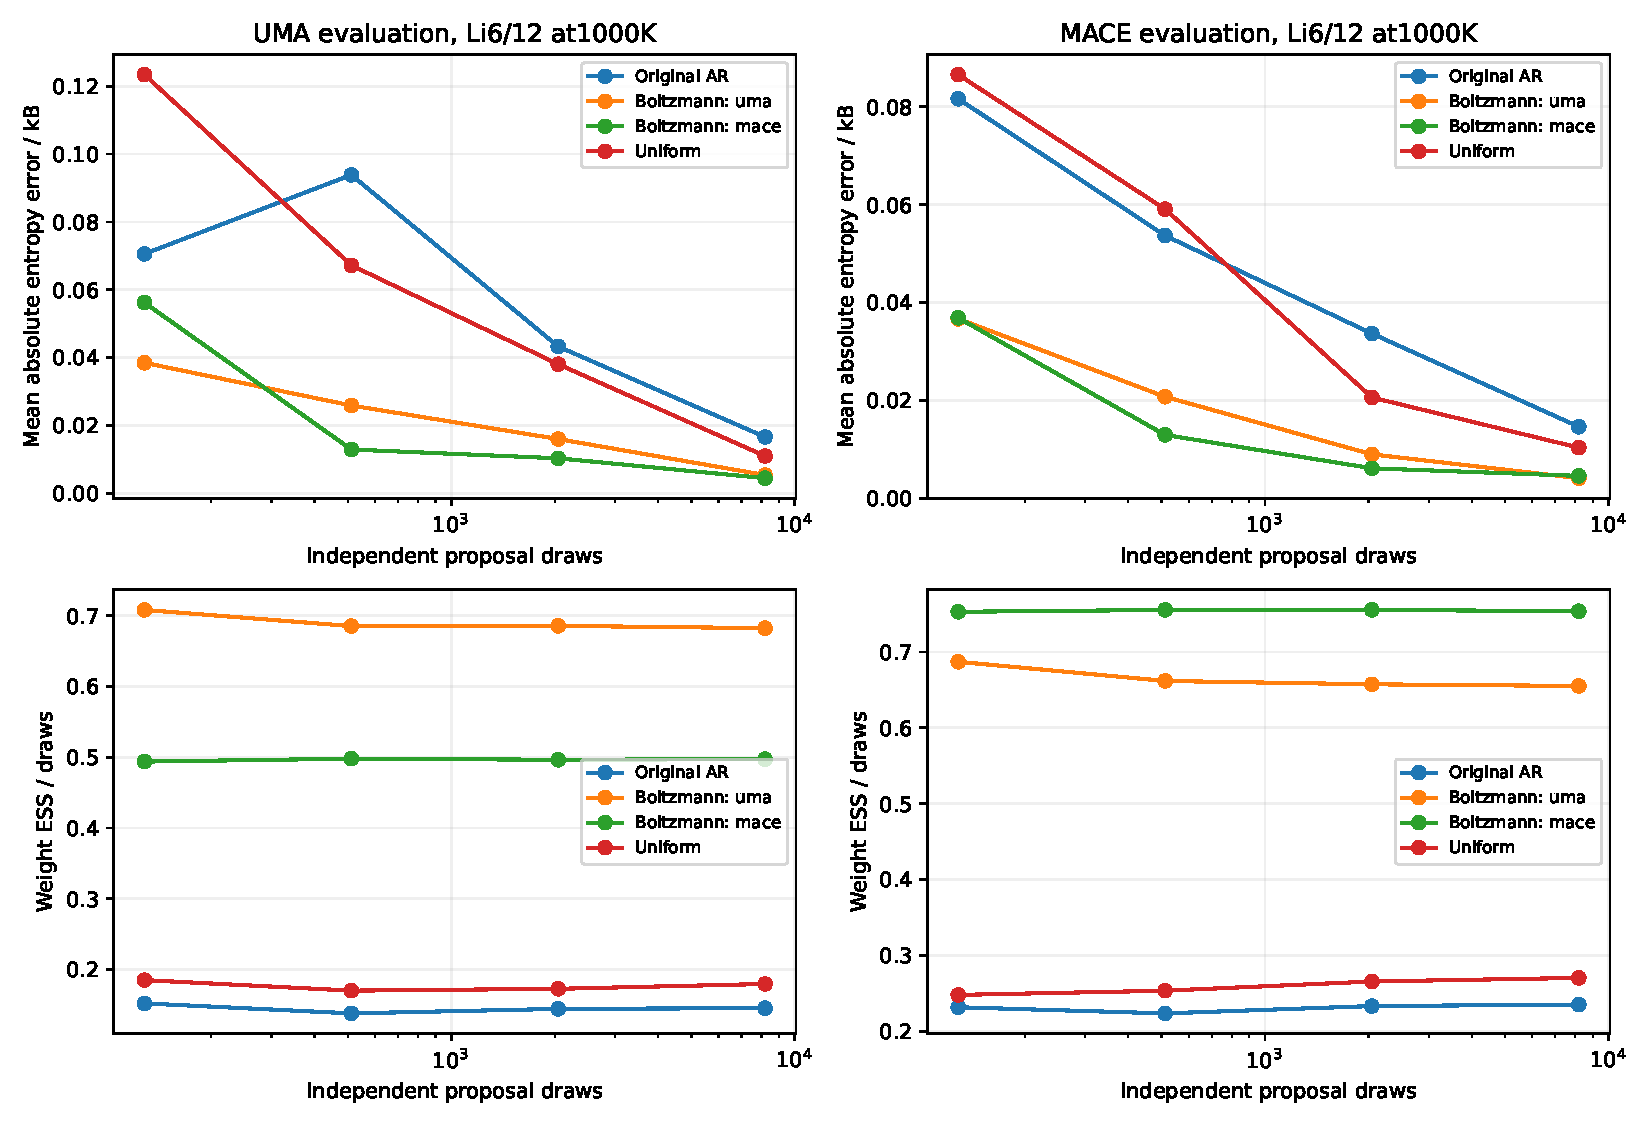
\includegraphics[width=\linewidth]{boltzmann_target_followup.pdf}
\caption{Li6/12 at 1,000 K: entropy MAE and weight ESS versus draw budget for
both teachers. The fixed-temperature training objective changes importance
efficiency without changing the reference. All sampled duplicates are retained.
Temperature transfer, including the negative 5,000 K result, is in the table.}
\end{figure}

A perfect Boltzmann proposal would make partition-sum importance weights
constant, minimizing their variance. That fact does not by itself minimize
finite-budget entropy error, which also contains the self-normalized energy
mean. We therefore evaluate entropy error and weight ESS separately. None of
these results turns the energy-bin-enriched N48 dataset into a density of
states: its adaptive selection law and novelty filtering differ from the
labelled-mask importance proposal used here.
